\chapter{Статические магнитоэлектрические эффекты}\label{ch:ch2}

В данной главе анализируются экспериментальные данные по магнитоэлектрической связи ионов меди и никеля в \ncbo, полученные в работах \cite{Nenert2007, Khanh2013} (см. \cref{sec:ch1/sec2}). Объясняется, почему авторы \cite{Nenert2007} не смогли обнаружить индукции электрической поляризации при переходе чистого \cbo\ в антиферромагнитную фазу и почему это удалось сделать в соединении, допированном ионами \niIon.

\section{Расчет расщепления состояний \cud\ и \nif\ кристаллическим полем}\label{sec:ch2/sec1}

Эффективность рассматриваемого нами далее механизма (см. \cref{sec:ch2/sec3}) зависит от особенностей энергетической структуры магнитного иона. Согласно структурным данным \cite{Martinez1971}, магнитные ионы \niIon и \cu занимают позиции с точечной группой симметрии \(S_4\) (рис. \cref{fig:cu_distributions}).

\begin{figure}[ht]
    \centerfloat{
        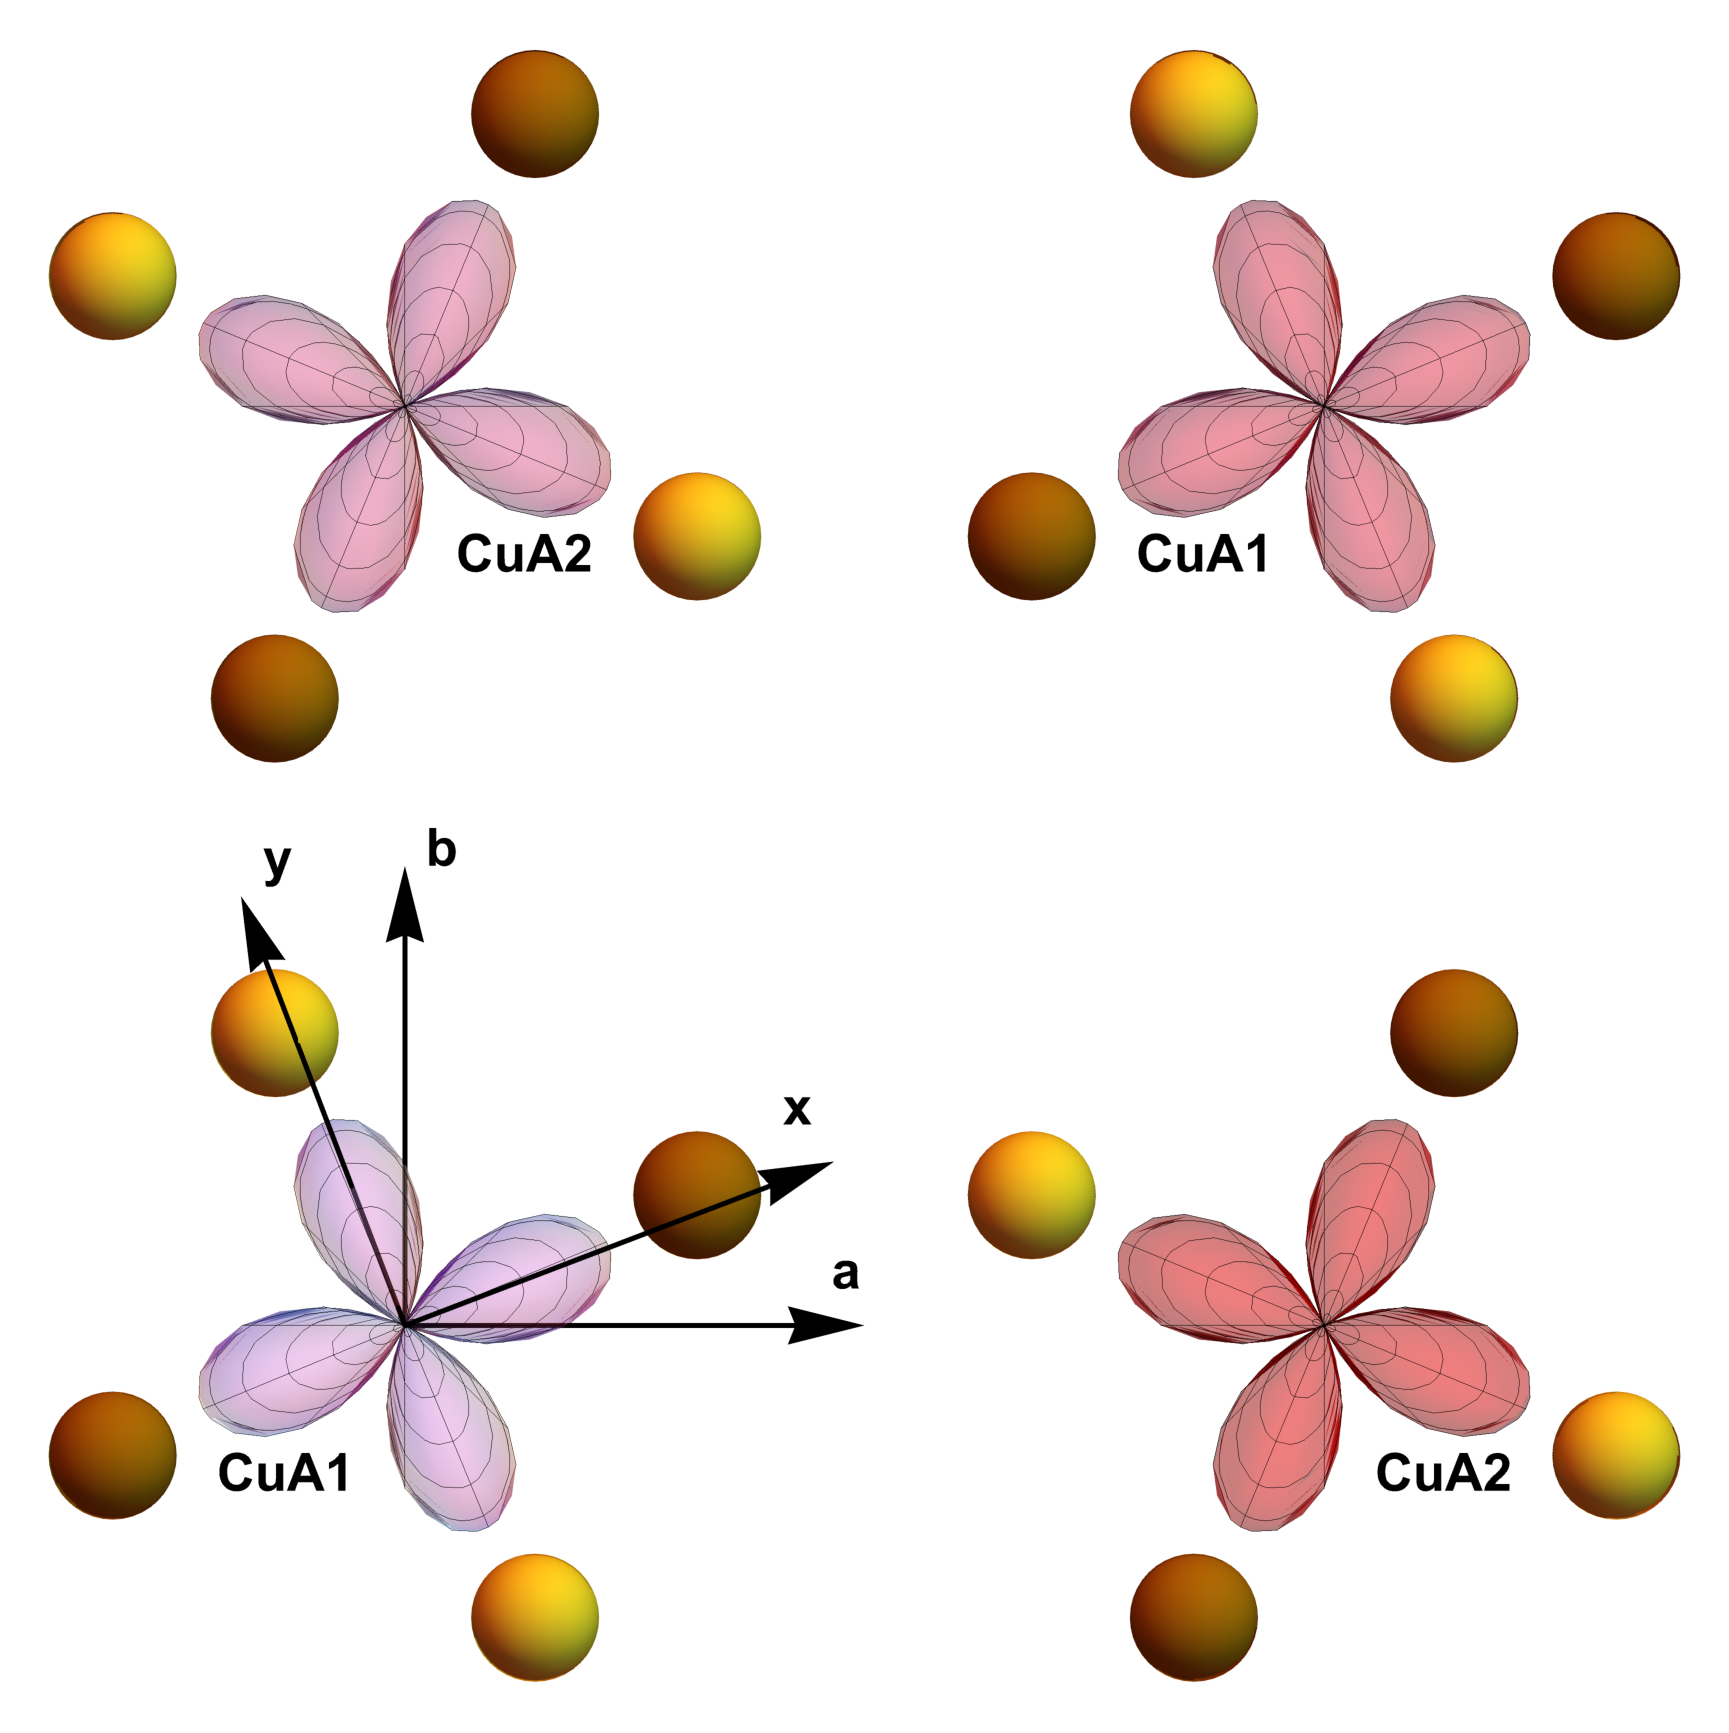
\includegraphics[scale=0.4]{cu_distributions}
    }
    \caption{Ортографическая проекция позиций элементарной ячейки подрешетки Cu 4b. Светло- и темно- желтым цветом изображены ионы кислорода, находящиеся соответственно выше и ниже по оси \textbf{c} относительно иона меди. Лепестки – рассчитанные нами распределения электронной плотности основных состояний ионов меди. \textit{a} и \textit{b} --- оси кристаллографической системы координат, \textit{x} и \textit{y} --- локальной оси локальной системы координат позиции A1. Насыщенность красного цвета в распределении электронной плотности меди соответствует увеличению координаты $z$ вдоль оси \textbf{c}, т.е. значениям $z\,{=}\,0,\,0.25,\,0.5 \text{ и } 0.75$ в единицах постоянных решетки в порядке увеличения яркости. Масштаб расстояний между позициями меди не соблюден.}
    \label{fig:cu_distributions}
\end{figure}

В этом случае оператор кристаллического поля имеет вид:

\begin{equation}
	\label{eq:Hcf}
	H_{cf}=B_{0}^{(2)}C_{0}^{(2)}+B_{0}^{(4)}C_{0}^{(4)}+B_{4}^{(4)}C_{4}^{(4)}+B_{-4}^{(4)}C_{-4}^{(4)},
\end{equation}

где $C_{q}^{(k)}$ - компоненты сферических тензорных операторов кристаллического поля, действующих на состояния 3d-электронов. Они связаны со сферическими функциями $Y_{k,q}\left( \theta,\phi \right)$ соотношением: $C_{q}^{(k)}=\sqrt{\frac{4\pi}{2k+1}}\sum Y_{k,q}\left( \theta_{i},\phi_{i} \right)$. Индекс суммирования $i$ относится к электронам в 3d-оболочке.

Ввиду того, что оба иона (\cu\ и \niIon) имеют одинаковый заряд, а при замещении меди никелем параметры кристаллической структуры в пределах погрешности не изменяются \cite{Khanh2013}, эти ионы имеют общий набор параметров кристаллического поля.
Эти параметры $B_{q}^{(k)}$ рассчитывались нами с использованием модели обменных зарядов \cite{Malkin1987}. Для оценки обменного заряда на связях никель-кислород привлекались экспериментальные данные о кристаллических расщеплениях \cu\ в \cbo, полученные в работе \cite{Pisarev2011}. Наша теоретико-групповая интерпретация возбужденных состояний соответствует интерпретации, предложенной Меньшениным \cite{Menshenin2017}. В локальной системе координат они оказались равными (в см$^{-1}$):

\begin{equation}
	\label{eq:CrystParams}
	B_{0}^{(2)}=-17720, B_{0}^{(4)}=9940, B_{4}^{(4)}=14030.
\end{equation}

Локальная система координат выбиралась из условия $Im\left[ B_{4}^{(4)} \right]=0$ и $Re\left[ B_{4}^{(4)} \right]>0$ --- для того, чтобы матрица оператора \cref{eq:Hcf} имела диагональный вид. Это означает, что для позиции \textit{A1} локальная система координат повернута относительно кристаллографической системы на угол \ang{20.9} вокруг оси с кристалла (угол отсчитывается против часовой стрелки), для позиции \textit{A2} угол поворота, соответственно равен минус \ang{20.9}. Интересно, что эти направления не совпадают с направлениями на соседние ионы кислорода из-за действия оинов более удаленных координационных сфер. Энергии кристаллических подуровней основного терма \cud\ и \nif\ и соответствующие им волновые функции приведены в таблицах \cref{tab:NiEnAndWf} и \cref{tab:CuEnAndWf} соответственно.

\begin{table} [htbp]% Пример записи таблицы с номером, но без отображаемого наименования
	\centering
	\begin{threeparttable}% выравнивание подписи по границам таблицы
		\caption{Уровни энергии и волновые функции \niIon\ в \nbo.}%
		\label{tab:NiEnAndWf}%
		\begin{SingleSpace}
			\begin{tabular}{| c | c | c |}
				\hline 
				Уровни энергии & Представления точечной & \multirow{2}{*}{Волновые функции} \\ 
				в см$^{-1}$ & группы $\mathrm{S}_{4}$ &  \\ 
				\hline 
				\multirow{2}{*}{13943} & \multirow{2}{*}{${ }^{2} \Gamma_{34}$} & $\psi_{7}=\mathrm{C}_{2}|-1\rangle+\mathrm{C}_{1}|3\rangle$ \\
				& & $\psi_{6}=\mathrm{C}_{2}|1\rangle+\mathrm{C}_{1}|-3\rangle$ \\
				\hline
				13768 & $\phantom{{ }^{2} }\Gamma_{1\phantom{4}}$ & $\psi_{5}=|0\rangle$ \\
				\hline
				11179 & ${ }^{2} \Gamma_{2\phantom{4}}$ & $\psi_{4}=\frac{1}{\sqrt{2}}(|2\rangle+|-2\rangle)$ \\
				\hline
				\multirow{2}{*}{4744} & \multirow{2}{*}{${ }^{1} \Gamma_{34}$} & $\psi_{3}=\mathrm{C}_{1}|-1\rangle-\mathrm{C}_{2}|3\rangle$ \\
				& & $\psi_{2}=\mathrm{C}_{1}|1\rangle-\mathrm{C}_{2}|-3\rangle$ \\
				\hline 0 & ${ }^{1} \Gamma_{2\phantom{4}}$ & $\psi_{1}=\frac{1}{\sqrt{2}}(|2\rangle-|-2\rangle)$ \\
				\hline
			\end{tabular}%
		\end{SingleSpace}
	\end{threeparttable}
\end{table}

\begin{table} [htbp]% Пример записи таблицы с номером, но без отображаемого наименования
	\centering
	\begin{threeparttable}% выравнивание подписи по границам таблицы
		\caption{Уровни энергии и волновые функции \cu\ в \cbo. В скобках указаны экспериментальные значения из \cite{Pisarev2011}.}%
		\label{tab:CuEnAndWf}%
		\begin{SingleSpace}
			\begin{tabular}{| c | c | c | c |}
				\hline 
				Уровни энергии & Представления точечной & \multirow{2}{*}{Волновые функции} \\ 
				в см$^{-1}$ & группы $\mathrm{S}_{4}$ &  \\ 
				\hline 
				15540 & \multirow{2}{*}{$\phantom{{ }^{2} }\Gamma_{34}$} & $\psi_{5}=\frac{i}{\sqrt{2}}(|-1\rangle+|1\rangle)$ \\
				(15440) & & $\psi_{4}=\frac{1}{\sqrt{2}}(|-1\rangle-|1\rangle)$ \\
				\hline
				13330 & \multirow{2}{*}{$\phantom{{ }^{2} }\Gamma_{1\phantom{4}}$} & \multirow{2}{*}{$\psi_{3}=|0\rangle$} \\
				(13450) & & \\
				\hline
				11170 & \multirow{2}{*}{${ }^{2} \Gamma_{2\phantom{4}}$} & \multirow{2}{*}{$\psi_{2}=\frac{i}{\sqrt{2}}(|-2\rangle-|2\rangle)$} \\
				(11340) & & \\
				\hline
				0 & ${ }^{1} \Gamma_{2\phantom{4}}$ & $\psi_{1}=\frac{1}{\sqrt{2}}(|2\rangle+|-2\rangle)$ \\
				\hline
			\end{tabular}%
		\end{SingleSpace}
	\end{threeparttable}
\end{table}

Значения коэффициентов в волновых функциях с точностью 1\% равны $C_{1}\cong\sqrt{\frac{1}{3}}, C_{2}\cong\sqrt{\frac{2}{3}}$. Как видно из таблиц 1 и 2, основным состоянием ионов никеля и меди является орбитальный синглет.

\section{Оператор связи орбитальных моментов 3d-электронов с электрическим полем}\label{sec:ch2/sec2}

Основное затруднение современной микроскопической теории динамической магнитоэлектрической связи связано с проблемой расчета электрических дипольных переходов. В этой связи в ранних работах \cite{Lovesey2009, Miyahara2012, Miyahara2014, Kezsmarki2014} ограничивались симметрийным анализом ненулевых компонент динамического магнитоэлектрического тензора. Известно, что в пределах состояний $3d$ оболочки электрические дипольные переходы запрещены законом сохранения четности. Уже давно в процессе исследований оптических спектров кристаллов было понято, что в позициях ионов без центра инверсии электрические дипольные переходы возникают из-за смешивания состояний основных электронных конфигураций $3d^n$ с возбужденными конфигурациями противоположной четности $3d^{n-1}4p$ \cite{Low1960}.

В случае редкоземельных соединений Джадд \cite{Judd1962} и Офельт \cite{Ofelt1962}, используя схему расчета во втором порядке теории возмущений, вывели удобные аналитические выражения для учета смешивания основных $4f^n$ электронных конфигураций с возбужденными $3f^{n-1}5d$ из-за нечетного кристаллического поля. Имеется большое число работ по применению результатов Джадда и Офельта, в которых отмечены достоинства и недостатки этой теории. В работах Корниенко с соавторами \cite{Kornienko1990, Dunina2008, Dunina2014} формулы работ \cite{Judd1962, Ofelt1962} дополнены членами высших порядков теории возмущений, которые позволили устранить принципиальные трудности теории Джадда-Офельта. 

В случае соединений с незаполненными $3d^n$ оболочками теория разработана сравнительно хуже. Проблема в том, что в области энергий возбужденных конфигураций $3d^{n-1}4p$ у элементов группы железа находятся также состояния с переносом электронов из $2p$ и $2s$ оболочек соседних ионов кислорода в незаполненную $3d$ оболочку и поэтому могут влиять на взаимодействие электронов с электрическим полем, как это отмечалось в \cite{Kornienko1977}. Расчеты, проведенные для \ce{LiCu2O2} \cite{Eremin2019jetp} и \ce{FeV2O4} \cite{Eremin2019prb}, с использованием накопленных данных магнитного резонанса о параметрах ковалентных связей, показали, что вклады в параметры эффективного электрического дипольного момента у ионов Сu$^{2+}$, Fe$^{2+}$, обусловленные виртуальными возбуждениями в состояния конфигурации $3d^{8}4p$ и в состояния с переносом заряда $\text{Cu}(3d^{10}) \, \text{O}(2p^{5})$ – одного порядка величины. 
Эффективный оператор связи c электрическим полем световой волны, учитывающий примешивание обеих возбужденных конфигураций к основной $3d^n$, имеет вид \cite{Eremin2019jetp, Eremin2019prb}:

\begin{equation}
	\label{eq:HE}
	\hat{H}_{E}=\sum_{k, p, t}\left\{E^{(1)} \hat{U}^{(k)}\right\}_{t}^{(p)} D_{t}^{(1 k) p},
\end{equation}

где фигурные скобки обозначают прямое произведение сферических компонент вектора электрического поля и единичного неприводимого тензорного оператора $\hat{U}^{(k)}$:

\begin{equation}
	\label{eq:electricalProduct}
	\left\{E^{(1)} \hat{U}^{(k)}\right\}_{t}^{(p)} = \sqrt{2p+1} \sum_{q,q^\prime} (-1)^{1-k+t} 
	\begin{pmatrix}
		1 & k & p \\
		q & q^\prime & -t
	\end{pmatrix}
	E_{q}^{(1)} \hat{U}_{q^\prime}^{(k)},
\end{equation}

\begin{equation}
	\label{eq:electricalComponents}
	E_{0}^{(1)} = E_z; \; E_{\pm 1}^{(1)} = \mp \frac{1}{\sqrt{2}} (E_x \pm i \cdot E_y).
\end{equation}

Индекс \textit{p}, в общем случае принимают нечетные значения 1, 3 и 5, а индекс \textit{k} – только четные 2 и 4. В модели суперпозиции, т. е. когда энергия системы считается равной сумме энергий отдельных пар, компоненты эффективного дипольного момента рассчитываются по следующей формуле:

\begin{equation}
	\label{eq:Deff}
	D^{(1k)p}_{t} = \sum_{j} d^{(1k)p}(R_j) \cdot (-1)^t \cdot C^{(p)}_{-t}(\theta_j,\phi_j),
\end{equation}

\begin{equation}
	\label{eq:d_contributions}
	d^{(1k)p}(R_j) = d^{(1k)p}_{cf}(R_j) + d^{(1k)p}_{cov}(R_j).
\end{equation}

Аналогично \cref{eq:Hcf}, индекс суммирования $j$ относится к электронам в 3d-оболочке. Первое слагаемое в \cref{eq:d_contributions}, учитывает действие внешнего электрического поля, усиленного нечетными кристаллическими полями от ионов решетки (как в теории Джадда--Офельта), а второе – влияние эффектов перекрывания электронных орбит меди с электронными облаками ионов кислорода и процессы переноса заряда (ковалентность). Явный вид формул для оценки величин параметров \cref{eq:d_contributions} приведен в работах \cite{Kornienko1977, Eremin2019jetp}.
Дополнительные правила отбора накладывает точечная группа симметрии $S_4$ позиций меди. В итоге нетрудно установить, что отличны от нуля следующие величины: $D_{\pm 2}^{(12)3}, \, D_{\pm 2}^{(14)3} \text{ и } D_{\pm 2}^{(14)5}$, которые имеют размерность электрического дипольного момента. Матричные элементы оператора $U^{(k)}$ рассчитываются через 3-\textit{j} символы:

\begin{equation}
	\label{eq:MatrixU}
	\langle dm_l \lvert \hat{U}_{q^\prime}^{(k)} \rvert dm_l^\prime \rangle = (-1)^{2-m_l} 
	\begin{pmatrix}
		2 & k & 2 \\
		-m_l & q^\prime & m_l^\prime
	\end{pmatrix}.
\end{equation}

В локальной системе координат для позиции A1 рассчитанные параметры \cref{eq:Deff} оказались равными (в а. е.):

\begin{equation}
	\label{eq:Dparams}
	\begin{array}{l}
		D_{2}^{(12) 3}=0.018+0.164 i   \\
		D_{2}^{(14) 3}=-0.110-0.055 i, \\
		D_{2}^{(14) 5}=-0.015-0.02 i
	\end{array}
\end{equation}

\section{Оператор связи спинов с электрическим полем}\label{sec:ch2/sec3}

Как уже подчёркивалось в экспериментальной работе \cite{Khanh2013}, особенности связи спинов \cu\ и \niIon\ c электрическим полем в этом соединении не могут быть объяснены ни моделью спиновых токов \cite{Katsura2005} ни стрикционным механизмом \cite{Sergienko2006}. Сами авторы работы \cite{Khanh2013} считали возможным объяснением механизм Аримы \cite{Arima2007}, однако, как будет показано далее, численные оценки эффекта, обусловленного этим механизмом на несколько порядков меньше наблюдающихся в эксперименте. К тому же, согласно этой гипотезе, основной вклад в поляризацию обусловлен ионами меди. В этой связи неясно --- почему в эксперименте с чистым боратом меди \cite{Nenert2007} поляризация не наблюдалась. 
В данном параграфе мы приводим результаты нашего расчета связи спинов с электрическим полем, которая индуцируется взаимодействием орбитальных моментов с электрическим полем и затем передается спин-орбитальным взаимодействием. Идея такого двухзвенного механизма, проиллюстрированного на рисунке \cref{fig:perturbation_model}, обсуждалась ранее в теории электрополевого эффекта магнитного резонанса в разбавленных парамагнетиках \cite{Mims}. Новизна нашего рассмотрения в этом плане связана с описанием первого звена, а именно природы связи 3d-электронов с электрическим полем (см. \cref{sec:ch2/sec2}). 

\begin{figure}[ht]
	\centerfloat{
		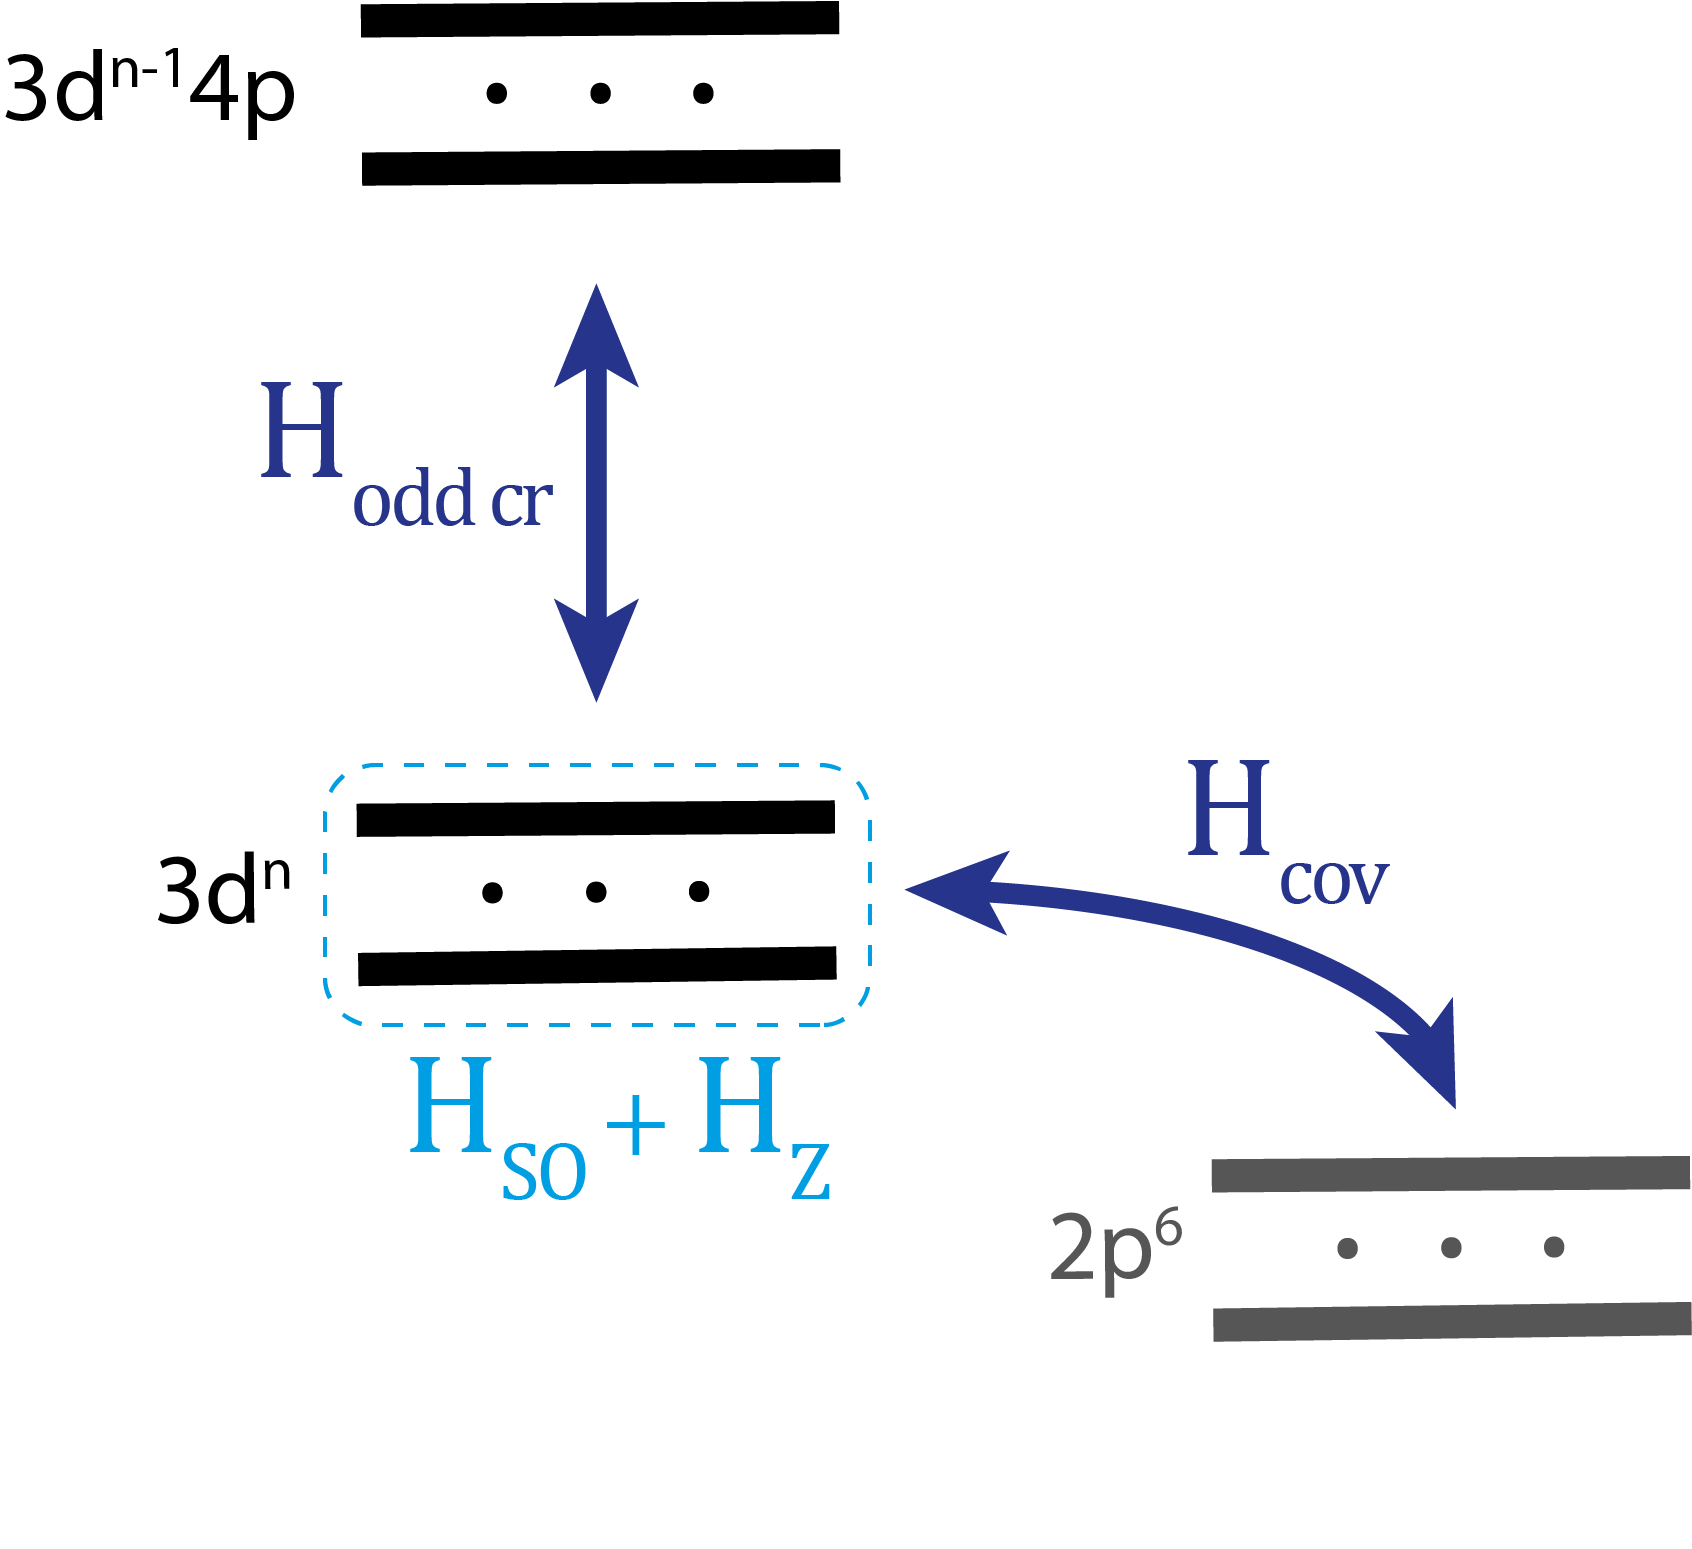
\includegraphics[scale=0.7]{perturbation_model}
	}
	\caption{Диаграмма, поясняющая механизм возникновения магнитоэлектрической связи. Взаимодействие орбитальных моментов с электрическим полем происходит благодаря примешиванию к основной конфигурации \(3d^n\) возбужденной конфигурации \(3d^{n-1}4p\) (за счет действия нечетного кристаллического поля), а также состояний с переносом заряда от лигандов O\(^{2-}\). Затем взаимодействие передается на спины  спин-орбитальным взаимодействием (в случае \cu окажется, что необходимо также зеемановское взаимодействие).}
	\label{fig:perturbation_model}
\end{figure}


\subsection{\nif}\label{subsec:ch2/sec3/sub1}

В третьем порядке теории возмущений имеются три типа процессов виртуальных возбуждений, приводящих к связи спинов с электрическим полем. Они поясняются на рис. \cref{fig:ni_trans}.

\begin{figure}[ht]
	\centerfloat{
		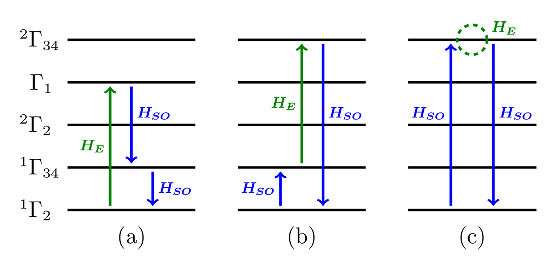
\includegraphics[scale=1.7]{ni_trans}
	}
	\caption{Схемы виртуальных возбуждений \nif.}
	\label{fig:ni_trans}
\end{figure}

В процессе возбуждения типа (a), из-за взаимодействия с электрическим полем (оператор $H_{E}$), происходит переход из основного состояния в возбужденное состояние $\Gamma_{1}$, затем из–за спин-орбитального взаимодействия в состояние $^{1}\Gamma_{34}$ и потом в основное $^{1}\Gamma_{2}$. При этом промежуточное состояние  $^{1}\Gamma_{34}$ может быть заменено на $^{2}\Gamma_{34}$. Учитывая также процессы сопряженные описанным (с противоположными направлениями стрелок) получаем эффективный оператор:

\begin{equation}
	\label{eq:NiHeffA}
	H_{eff}^{(a)}=i \frac{\lambda_{Ni}^{2} D_{z}^{(a)}}{E\left(\Gamma_{1}\right)}\left(\frac{C_{1}\left(\sqrt{15} C_{1}+3 C_{2}\right)}{E\left(1 \Gamma_{34}\right)}+\frac{C_{2}\left(\sqrt{15} C_{2}-3 C_{1}\right)}{E\left(2 \Gamma_{34}\right)}\right)\left(S_{+}^{2}-S_{-}^{2}\right) E_{z},
\end{equation}

где $S_{+}$ и $S_{-}$ – операторы повышения и понижения спина соответственно и введено следующее обозначение:

\begin{equation}
	\label{eq:NiDzA}
	D_{z}^{(a)}=\operatorname{Im}\left[\frac{1}{5} \sqrt{\frac{1}{21}} D_{-2}^{(12) 3}-\frac{1}{6} \sqrt{\frac{1}{35}} D_{-2}^{(14) 3}+\frac{1}{30} D_{-2}^{(14) 5}\right].
\end{equation}

На рис. \cref{fig:ni_trans}b изображен второй возможный процесс: возбуждение вначале индуцируется спин-орбитальным взаимодействием (оператор $H_{SO}$) на $^{1}\Gamma_{2}$, затем происходит переход из-за взаимодействия с электрическим полем на состояние $^{2}\Gamma_{34}$ и на третьем этапе под действием спин-орбитального взаимодействия – в основное состояние $^{1}\Gamma_{2}$. Соответствующий этому типу процессов оператор связи спинов с электрическим полем записывается следующим образом:

\begin{equation}
	\label{eq:NiHeffB}
	\begin{aligned}
		H_{eff}^{(b)} & =\frac{\lambda_{Ni}^{2}\left(\sqrt{5} C_{1}+\sqrt{3} 	C_{2}\right)\left(\sqrt{3} C_{1}-\sqrt{5} C_{2}\right)}{2 E\left({ }^{1} \Gamma_{34}\right) E\left({ }^{2} \Gamma_{34}\right)} \times \\
		& \times \left(\left(S_{+}^{2}+S_{-}^{2}\right) 	\operatorname{Re}\left[D_{z}^{(b)}\right]+i\left(S_{+}^{2}-S_{-}^{2}\right) \operatorname{Im}\left[D_{z}^{(b)}\right]\right) E_{z},
	\end{aligned}
\end{equation}

\begin{equation}
	\label{eq:NiDzB}
	\begin{aligned}
		D_{z}^{(b)} & =\left(C_{1}^{2}-C_{2}^{2}\right)\left[-\frac{1}{5} \sqrt{\frac{1}{21}} D_{2}^{(12) 3}-\sqrt{\frac{1}{35}} D_{2}^{(14) 3} +\frac{1}{5} D_{2}^{(14) 5}\right] + \\
		& + C_{1} C_{2}\left[-\frac{2}{5} \sqrt{\frac{1}{35}} D_{-2}^{(12) 3}+\frac{2}{3} \sqrt{\frac{1}{21}} D_{-2}^{(14) 3}-\frac{2}{3} \sqrt{\frac{1}{15}} D_{-2}^{(14) 5}\right].
	\end{aligned}
\end{equation}

Третий тип процессов на рис. \cref{fig:ni_trans}c реализуется через  орбитально вырожденные состояния $^{2}\Gamma_{34}$ (а также через  $^{1}\Gamma_{34}$), в базисе которых имеются матричные элементы от оператора $H_{E}$.  Соответствующий оператор связи спинов с электрическим полем записывается в виде:

\begin{equation}
	\label{eq:NiHeffC}
	\begin{aligned}
		& H_{eff}^{(c)}=  -\frac{\lambda_{Ni}^{2}}{4}\left(\frac{\left(\sqrt{5} C_{1}+\sqrt{3} C_{2}\right)^{2}\left(\left(S_{+}^{2}+S_{-}^{2}\right) \operatorname{Re}\left[D_{z}^{\left(c_{1}\right)}\right]+i\left(S_{+}^{2}-S_{-}^{2}\right) \operatorname{Im}\left[D_{z}^{\left(c_{1}\right)}\right]\right)}{E\left({ }^{1} \Gamma_{34}\right)^{2}}\right. \\
		& \left.+\frac{\left(\sqrt{3} C_{1}-\sqrt{5} C_{2}\right)^{2}\left(\left(S_{+}^{2}+S_{-}^{2}\right) \operatorname{Re}\left[D_{z}^{\left(c_{2}\right)}\right]+i\left(S_{+}^{2}-S_{-}^{2}\right) \operatorname{Im}\left[D_{z}^{\left(c_{2}\right)}\right]\right)}{E\left({ }^{2} \Gamma_{34}\right)^{2}}\right) E_{z},
	\end{aligned}
\end{equation}

где введены обозначения:
\begin{equation}
	\label{eq:NiDzC}
	\begin{aligned}
		D_{z}^{\left(c_{1}\right)} & = C_{1}^{2}D_{1}+C_{1} C_{2}D_{2}, \\
		D_{z}^{\left(c_{2}\right)} & = C_{2}^{2}D_{1}-C_{1} C_{2}D_{2},\\
		D_{1} & = -\frac{2}{5} \sqrt{\frac{1}{35}} D_{-2}^{(12) 3}+\frac{2}{3} \sqrt{\frac{1}{21}} D_{-2}^{(14) 3}-\frac{2}{3} \sqrt{\frac{1}{15}} D_{-2}^{(14) 5}, \\
		D_{2} & = \frac{2}{5} \sqrt{\frac{1}{21}} D_{2}^{(12) 3}+2 \sqrt{\frac{1}{35}} D_{2}^{(14) 3}-\frac{2}{5} D_{2}^{(14) 5}.
	\end{aligned}
\end{equation}

\subsection{\cud}\label{subsec:ch2/sec3/sub2}

Отметим, что описанные выше операторы можно рассмотреть и в случае иона \cud\ для соединения \cbo. Однако, как нетрудно убедиться, для ионов с $S=1/2$ все матричные элементы операторов $S_{+}^{2}$ и $S_{-}^{2}$ равны нулю. Это объясняет резкое усиление связи спинов с электрическим полем в кристаллах \cbo\ при замене ионов Cu$^{2+}$($^{2}$D) на ионы Ni$^{2+}$($^{3}$F), обнаруженное в работе \cite{Khanh2013}.

\begin{figure}[ht]
	\centerfloat{
		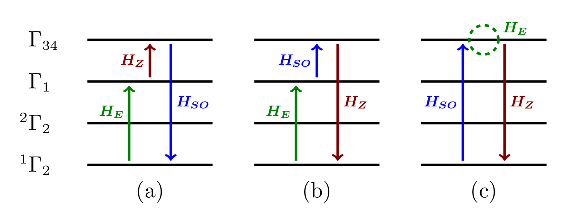
\includegraphics[scale=1.7]{cu_trans}
	}
	\caption{Схемы виртуальных возбуждений \cud.}
	\label{fig:cu_trans}
\end{figure}

Происхождение магнитоэлектрической связи мы можем также объяснить виртуальными процессами возбуждения иона меди (поясняются на рис. \cref{fig:cu_trans}). Комбинируя в третьем порядке теории возмущений операторы $H_{E}$, $H_{SO}$ и оператор взаимодействия орбитального момента меди с индукцией магнитного поля, получаем эффективный оператор энергии связи:

\begin{equation}
	\label{eq:CuHEff}
	H_{eff}^{Cu}=\frac{\lambda_{Сu} \mu_{B} d_{z}^{(a)}}{E\left(\Gamma_{1}\right) E\left(\Gamma_{34}\right)}\left[S_{+} B_{+}+S_{-} B_{-}\right] E_{z} - \frac{\lambda_{Cu} \mu_{B} }{2 E\left(\Gamma_{34}\right)^{2}}\left[d_{z_{-}}^{(b)}S_{+} B_{+} + d_{z_{+}}^{(b)} S_{-} B_{-}\right] E_{z},
\end{equation}

где $B_{+}=B_{x}+iB_{y}, B_{-}=B_{x}-iB_{y}$, а параметры, описывающие связь 3d-электронов с электрическим полем, определяются выражениями:

\begin{equation}
	\label{eq:CuDz}
	\begin{aligned}
		d_{z}^{(a)}&=\operatorname{Re}\left[-2 \sqrt{\frac{1}{35}} D_{2}^{(12) 3}+\sqrt{\frac{1}{21}} D_{2}^{(14) 3}-\sqrt{\frac{1}{15}} D_{2}^{(14) 5}\right], \\
		d_{z_{\pm}}^{(b)}&=\sqrt{\frac{1}{35}} D_{\pm2}^{(12)3}+\frac{2}{3} \sqrt{\frac{1}{21}} D_{\pm2}^{(14) 3}-\frac{2}{3} \sqrt{\frac{1}{15}} D_{\pm2}^{(14) 5}.
	\end{aligned}
\end{equation}

\subsection{Анализ полученных операторов и обсуждение результатов}\label{subsec:ch2/sec3/sub3}

Из выражений \cref{eq:NiHeffA, eq:NiHeffB, eq:NiHeffC} видно,что спонтанное упорядочение спинов \niIon в плоскости ab кристалла индуцирует возникновение электрической поляризации вдоль оси \textit{с}. Этот результат нашего расчета соответствует экспериментальным данным \cite{Khanh2013}. Далее перейдем к численным оценкам входящих в \cref{eq:NiHeffA, eq:NiHeffB, eq:NiHeffC} величин.

Подставляя \cref{eq:Dparams} в \cref{eq:NiDzA, eq:NiDzB, eq:NiDzC}, получаем (в а. е.): $D_{z}^{(a)}=-0.006$, $D_{z}^{(b)}=-0.012+0.007 i$, $D_{z}^{\left(c_{1}\right)}=-0.019+0.016 i$, $D_{z}^{\left(c_{2}\right)}=0.004-0.013 i$. Используя эти величины и значения энергетических интервалов из таблицы \cref{tab:NiEnAndWf}, по формулам \cref{eq:NiHeffA, eq:NiHeffB, eq:NiHeffC} получаем вид оператора связи спинов никеля c электрическим полем в расчёте на один ион \niIon:
\begin{equation}
	\label{eq:NiHeffSum}
	H_{eff}^{Ni}=d_{1}^{Ni}\left(S_{+}^{2}+S_{-}^{2}\right) E_{z}+i d_{2}^{Ni}\left(S_{+}^{2}-S_{-}^{2}\right) E_{z},
\end{equation}
где $d_{1}^{Ni}=0.00114$ а. е., $d_{2}^{Ni}=-0.00115$ а. е.

Умножив эти значения на концентрацию ионов в позиции 4b ($N\mathop{=}2.54\mathop{\cdot}10^{21} см^{-3}$), получаем коэффициенты макроскопической электрической поляризации $P_{1}=d_{1}^{Ni}N=24.4$ мкКл/м$^{2}$, $P_{2}=d_{2}^{Ni}N=-24.7$ мкКл/м$^{2}$.

Напомним, что максимальное значение макроскопической электрической поляризации в \ncbo, зарегистрированное в работе \cite{Khanh2013} равно 3.5 мкКл/м$^{2}$ для концентрации никеля 2.7\%.

Таким образом, мы убеждаемся, что рассмотренный нами механизм вполне объясняет происхождение связи спинов иона никеля c электрическим полем. 

Что касается механизма Аримы \cite{Arima2007}, то его можно оценить следующим образом: в формулах \cite{Arima2007} также, как и в \cref{eq:NiHeffA, eq:NiHeffB, eq:NiHeffC} фигурирует параметр спин-орбитальной связи, умноженный на квадрат коэффициента перед антисвязывающей орбиталью ($\lambda_{\sigma}\sim0.2$). При этом, вместо энергии возбуждения иона Ni в формулах \cref{eq:NiHeffA, eq:NiHeffB, eq:NiHeffC} будет фигурировать энергия переноса заряда из 2p- оболочки кислорода в 3d- оболочку никеля, а это примерно 80000 см$^{-1}$ \cite{Simonetti1977}. Кроме того, в формулах Аримы \cite{Arima2007} не принимается во внимание фактор усиления действия электрического поля на орбитальный момент 3d- электрона, связанный с нечетным кристаллическим полем. Суммируя сказанное, приходим к выводу, что параметр связи спина с электрическим полем по механизму Аримы примерно на 2-3 порядка меньше измеренного в \ncbo\ и может быть отброшен не только в случае \ncbo, но и в других оксидах с незаполненными 3d-оболочками.

Как отмечалось выше, связь спинов меди с электрическим полем по механизмам \cref{eq:NiHeffA, eq:NiHeffB, eq:NiHeffC} отсутствует. Этот вывод соответствует результатам работы \cite{Nenert2007}, в которой магнитоэлектрическая связь в \cbo\ не была обнаружена, хотя для этого предпринимались специальные исследования. Позже в работе \cite{Toyoda2016} сообщалось, что электрическая поляризация в \cbo\ вдоль оси с кристалла возникает, если приложить внешнее магнитное поле в плоскости ab. 

Из \cref{eq:CuHEff} видно, что индукция магнитного поля \textbf{B}, лежащая в плоскости \textit{ab} индуцирует электрическую поляризацию вдоль оси \textit{с} кристалла. Перепишем \cref{eq:CuHEff}, используя аналогичные \cref{eq:NiHeffSum} обозначения:

\begin{equation}
	\label{eq:CuHeffSum}
	H_{eff}^{Cu}=d_{1}^{Cu} \left[S_{+} B_{+}+S_{-} B_{-}\right] E_{z} + i d_{2}^{Cu}\left[S_{-} B_{-}-S_{+} B_{+}\right] E_{z},
\end{equation}

где $d_{1}^{Cu}=3.9\cdot10^{-8}$ а. е., $d_{2}^{Cu}=2.8\cdot10^{-8}$ а. е.
Коэффициенты макроскопической электрической поляризации в \cbo\, индуцированной внешним магнитным полем в плоскости ab равны: $P_{1}^{Cu}\mathop{=}d_{1}^{Cu}N\mathop{=}0.0008$ мкКл/Тл$\mathop{\cdot}$м$^{2}$, $P_{2}^{Cu}\mathop{=}d_{2}^{Cu}N\mathop{=}0.0006$ мкКл/Тл$\mathop{\cdot}$м$^{2}$.
Таким образом поляризация может проявиться лишь в сильных магнитных полях порядка 10 Тл, либо при допировании \cbo\  редкоземельными ионами с большими магнитными моментами, как это происходит в  кристаллах \ce{DyCrO4} \cite{Eremin2020}.

\FloatBarrier
